\section{Tanda Tangan Digital}
Tanda tangan digital bukanlah salinan digital dari tanda tangan basah,
melainkan sebuah mekanisme kriptografis yang mengikat identitas pengirim
dengan isi pesan. Tanda tangan basah \emph{melekat pada kertas}, bukan pada
tulisan: pemindahan tulisan ke lembar lain memindahkan tulisan tanpa
tanda tangan itu. Tanda tangan digital dirancang justru untuk menutup celah
tersebut. Nilainya dihitung dari isi pesan, sehingga perubahan sekecil satu
bit pun membuat nilai itu tidak lagi cocok. Inilah perbedaan mendasar yang
membuat tanda tangan digital dapat diperiksa mesin, sedangkan tanda tangan
basah tidak \citep{stallings2017}.

\subsection{Mekanisme Kerja Tanda Tangan Digital}
Berbeda dengan enkripsi pesan (di mana pesan dienkripsi dengan kunci publik
penerima), tanda tangan digital dibuat menggunakan \textbf{kunci privat
pengirim}. Perhatikan arah pemakaian kuncinya, karena inilah inti perbedaan
tanda tangan dari enkripsi:

\begin{itemize}
    \item \textbf{Enkripsi}: siapa pun dapat memakai kunci publik penerima
          untuk mengunci pesan, tetapi hanya pemilik kunci privat penerima
          yang dapat membukanya. Kunci publik bersifat terbuka, jadi tidak
          ada yang istimewa pada kemampuan mengunci.
    \item \textbf{Tanda tangan}: hanya satu pihak yang dapat menandai pesan,
          yaitu pemilik kunci privatnya, tetapi siapa pun dapat memakai kunci
          publiknya untuk memeriksa tanda tangan itu. Di sini justru
          kemampuannya memeriksa yang bersifat terbuka.
\end{itemize}

\textbf{Proses Penandatanganan (Signing):}
\begin{enumerate}
    \item Pengirim membuat \textit{hash} dari pesan asli: $h = \text{Hash}(M)$.
    \item Pengirim mengenkripsi nilai hash tersebut menggunakan kunci privatnya:
          $S = E_{K_{priv}}(h)$.
    \item Pesan $M$ dan tanda tangan $S$ dikirimkan kepada penerima.
\end{enumerate}

\textbf{Proses Verifikasi (Verification):}
\begin{enumerate}
    \item Penerima menghitung hash dari pesan $M$ yang diterima: $h' = \text{Hash}(M)$.
    \item Penerima mendekripsi tanda tangan $S$ menggunakan kunci publik pengirim:
          $h = D_{K_{pub}}(S)$.
    \item Jika $h = h'$, maka tanda tangan valid. Ini membuktikan dua hal:
    \begin{itemize}
        \item \textbf{Integritas}: Pesan tidak berubah sejak ditandatangani.
        \item \textbf{Otentikasi}: Pesan benar-benar berasal dari pemilik kunci
              privat tersebut.
    \end{itemize}
\end{enumerate}

% Alur penandatanganan dan verifikasi tanda tangan digital.
% Dirujuk dari section-02.tex dengan % Alur penandatanganan dan verifikasi tanda tangan digital.
% Dirujuk dari section-02.tex dengan % Alur penandatanganan dan verifikasi tanda tangan digital.
% Dirujuk dari section-02.tex dengan \input{figures/alur-tanda-tangan}.
\begin{figure}[htbp]
    \centering
    \begin{tikzpicture}[
        kotak/.style={draw, rounded corners, align=center, font=\small, inner sep=4pt,
                      minimum height=0.8cm},
        panah/.style={-{Latex[length=2mm]}, thick},
    ]
        % ---------- Penandatanganan ----------
        \node[font=\small\bfseries] at (2.8,0.85) {Penandatanganan (oleh pengirim)};
        \node[kotak, fill=blue!6, minimum width=1.4cm] (m1) at (0,0) {$M$};
        \node[kotak, fill=orange!12, minimum width=1.8cm] (h1) at (2.0,0) {Hash};
        \node[kotak, fill=gray!8, minimum width=2.4cm] (e1) at (4.4,0) {$E_{K_{priv}}$};
        \node[kotak, fill=green!10, minimum width=1.8cm] (s1) at (7.0,0) {$S$};
        \draw[panah] (m1) -- (h1);
        \draw[panah] (h1) -- node[above, font=\scriptsize] {$h$} (e1);
        \draw[panah] (e1) -- (s1);

        % ---------- Verifikasi ----------
        \node[font=\small\bfseries] at (2.8,-1.75) {Verifikasi (oleh penerima)};
        \node[kotak, fill=blue!6, minimum width=1.4cm] (m2) at (0,-2.6) {$M$};
        \node[kotak, fill=orange!12, minimum width=1.8cm] (h2) at (2.0,-2.6) {Hash};
        \node[kotak, fill=blue!6, minimum width=1.4cm] (s2) at (0,-4.0) {$S$};
        \node[kotak, fill=gray!8, minimum width=2.4cm] (d2) at (2.0,-4.0) {$D_{K_{pub}}$};
        \node[kotak, fill=yellow!18, minimum width=2.6cm] (cmp) at (5.6,-3.3) {$h' = h$?};

        \draw[panah] (m2) -- (h2);
        \draw[panah] (s2) -- (d2);
        \draw[panah] (h2) -- node[above, font=\scriptsize] {$h'$} (cmp);
        \draw[panah] (d2) -- node[below, font=\scriptsize] {$h$} (cmp);
    \end{tikzpicture}
    \caption{Alur tanda tangan digital: penandatanganan memakai kunci privat pengirim, verifikasi memakai kunci publiknya}
    \label{fig:alur-tanda-tangan}
\end{figure}
.
\begin{figure}[htbp]
    \centering
    \begin{tikzpicture}[
        kotak/.style={draw, rounded corners, align=center, font=\small, inner sep=4pt,
                      minimum height=0.8cm},
        panah/.style={-{Latex[length=2mm]}, thick},
    ]
        % ---------- Penandatanganan ----------
        \node[font=\small\bfseries] at (2.8,0.85) {Penandatanganan (oleh pengirim)};
        \node[kotak, fill=blue!6, minimum width=1.4cm] (m1) at (0,0) {$M$};
        \node[kotak, fill=orange!12, minimum width=1.8cm] (h1) at (2.0,0) {Hash};
        \node[kotak, fill=gray!8, minimum width=2.4cm] (e1) at (4.4,0) {$E_{K_{priv}}$};
        \node[kotak, fill=green!10, minimum width=1.8cm] (s1) at (7.0,0) {$S$};
        \draw[panah] (m1) -- (h1);
        \draw[panah] (h1) -- node[above, font=\scriptsize] {$h$} (e1);
        \draw[panah] (e1) -- (s1);

        % ---------- Verifikasi ----------
        \node[font=\small\bfseries] at (2.8,-1.75) {Verifikasi (oleh penerima)};
        \node[kotak, fill=blue!6, minimum width=1.4cm] (m2) at (0,-2.6) {$M$};
        \node[kotak, fill=orange!12, minimum width=1.8cm] (h2) at (2.0,-2.6) {Hash};
        \node[kotak, fill=blue!6, minimum width=1.4cm] (s2) at (0,-4.0) {$S$};
        \node[kotak, fill=gray!8, minimum width=2.4cm] (d2) at (2.0,-4.0) {$D_{K_{pub}}$};
        \node[kotak, fill=yellow!18, minimum width=2.6cm] (cmp) at (5.6,-3.3) {$h' = h$?};

        \draw[panah] (m2) -- (h2);
        \draw[panah] (s2) -- (d2);
        \draw[panah] (h2) -- node[above, font=\scriptsize] {$h'$} (cmp);
        \draw[panah] (d2) -- node[below, font=\scriptsize] {$h$} (cmp);
    \end{tikzpicture}
    \caption{Alur tanda tangan digital: penandatanganan memakai kunci privat pengirim, verifikasi memakai kunci publiknya}
    \label{fig:alur-tanda-tangan}
\end{figure}
.
\begin{figure}[htbp]
    \centering
    \begin{tikzpicture}[
        kotak/.style={draw, rounded corners, align=center, font=\small, inner sep=4pt,
                      minimum height=0.8cm},
        panah/.style={-{Latex[length=2mm]}, thick},
    ]
        % ---------- Penandatanganan ----------
        \node[font=\small\bfseries] at (2.8,0.85) {Penandatanganan (oleh pengirim)};
        \node[kotak, fill=blue!6, minimum width=1.4cm] (m1) at (0,0) {$M$};
        \node[kotak, fill=orange!12, minimum width=1.8cm] (h1) at (2.0,0) {Hash};
        \node[kotak, fill=gray!8, minimum width=2.4cm] (e1) at (4.4,0) {$E_{K_{priv}}$};
        \node[kotak, fill=green!10, minimum width=1.8cm] (s1) at (7.0,0) {$S$};
        \draw[panah] (m1) -- (h1);
        \draw[panah] (h1) -- node[above, font=\scriptsize] {$h$} (e1);
        \draw[panah] (e1) -- (s1);

        % ---------- Verifikasi ----------
        \node[font=\small\bfseries] at (2.8,-1.75) {Verifikasi (oleh penerima)};
        \node[kotak, fill=blue!6, minimum width=1.4cm] (m2) at (0,-2.6) {$M$};
        \node[kotak, fill=orange!12, minimum width=1.8cm] (h2) at (2.0,-2.6) {Hash};
        \node[kotak, fill=blue!6, minimum width=1.4cm] (s2) at (0,-4.0) {$S$};
        \node[kotak, fill=gray!8, minimum width=2.4cm] (d2) at (2.0,-4.0) {$D_{K_{pub}}$};
        \node[kotak, fill=yellow!18, minimum width=2.6cm] (cmp) at (5.6,-3.3) {$h' = h$?};

        \draw[panah] (m2) -- (h2);
        \draw[panah] (s2) -- (d2);
        \draw[panah] (h2) -- node[above, font=\scriptsize] {$h'$} (cmp);
        \draw[panah] (d2) -- node[below, font=\scriptsize] {$h$} (cmp);
    \end{tikzpicture}
    \caption{Alur tanda tangan digital: penandatanganan memakai kunci privat pengirim, verifikasi memakai kunci publiknya}
    \label{fig:alur-tanda-tangan}
\end{figure}


Rumus di atas dituliskan dengan lambang $E$ dan $D$ karena pada kenyataannya
tanda tangan RSA memang operasi eksponen yang sama dengan enkripsi RSA, hanya
saja urutan pemakaian kuncinya terbalik. Penulisan seperti itu memiliki satu
bahaya: ia tidak berlaku untuk semua skema tanda tangan. Pada DSA dan ECDSA
tidak ada ``dekripsi'' sama sekali --- yang ada hanyalah pemeriksaan
kecocokan persamaan. Karena itu skema tanda tangan modern lebih tepat
dirumuskan sebagai sepasang prosedur $(\mathrm{Sign}, \mathrm{Verify})$ yang
tidak menuntut sifat dapat dibalik.

\subsection{Sifat Keamanan yang Dituntut}
\label{subsec:sifat-tanda-tangan}
Sebuah skema tanda tangan yang baik dituntut memenuhi dua sifat pokok
\citep{katz2020}.

\textbf{1. Tidak dapat dipalsukan} (\textit{unforgeability}). Tanpa kunci
privat penanda tangan, tidak ada pihak lain yang dapat menghasilkan pasangan
pesan dan tanda tangan yang diterima oleh prosedur verifikasi. Model ancaman
baku untuk sifat ini disebut \emph{EUF-CMA}, singkatan dari
\textit{existential unforgeability under chosen-message attack}. Artinya,
penyerang bahkan diizinkan meminta tanda tangan sah atas pesan apa pun yang
ia pilih --- misalnya karena ia menyadap banyak dokumen bertanda tangan ---
dan tetap harus tidak mampu membuat tanda tangan untuk pesan baru, sekecil
apa pun peluang keberhasilannya. Perhatikan bahwa ``pesan baru'' tidak harus
bermakna bagi penyerang; keluarganya saja sudah cukup untuk menyebut serangan
itu berhasil. Model yang lebih ketat, \emph{strong unforgeability},
menuntut penyerang bahkan tidak dapat membuat tanda tangan \emph{kedua} atas
pesan yang sudah pernah ditandatangani.

\textbf{2. Tidak dapat dialihkan} (\textit{non-transferability} atau
\emph{non-malleability}, dalam arti ketat). Sifat ini berkaitan dengan
serangan \textit{malleability} (kelenturan): bila dari tanda tangan yang sah
penyerang dapat menurunkan tanda tangan sah yang lain atas pesan yang
berbeda, skema tersebut rusak. Bentuk paling sederhana muncul pada RSA
``buku teks'' yang dibahas di bawah.

Dua sifat itu belum menyebut kerahasiaan. Tanda tangan tidak menyembunyikan
apa pun; ia hanya membuktikan keaslian. Perlu ditegaskan pula bahwa
verifikasi tanda tangan bersifat \emph{publik dan berulang}: siapa pun dapat
memeriksa tanda tangan yang sama sebanyak apa pun tanpa merusaknya. Sifat ini
berbeda dari kata sandi yang sebaiknya sekali pakai, dan justru inilah yang
membuat non-repudiation mungkin.

\subsection{Mengapa Pesan Di-hash Lebih Dulu}
Fungsi hash memampatkan pesan berukuran berapa pun menjadi nilai ringkas
berukuran tetap lebih kecil dari modulus. Tanpa hashing, tanda tangan pada
pesan panjang menjadi mahal (RSA hanya bekerja pada satu elemen modulo $n$),
dan skema seperti DSA/ECDSA tidak dapat menandatangani pesan mentah. Hashing
juga mengikat tanda tangan pada pesan: penggantian pesan oleh penyerang
menuntut ditemukannya kolisi, yang praktis mustahil untuk SHA-256
\citep{katz2020}.

Angka-angka pada Bab~15 dapat dipakai untuk mengukur tuntutan ini. Sebuah
pesan 10 MB perlu dipotong menjadi blok-blok seukuran modulus RSA; untuk
RSA-3072, modulusnya hanya 384 byte, sehingga pesan itu terbagi menjadi lebih
dari $27.000$ blok, dan menandatangani tiap blok berarti $27.000$ operasi
eksponen modular yang masing-masing berbiaya jutaan perkalian bit. Dengan
hashing, seluruh 10 MB diringkas menjadi 32 byte terlebih dahulu, dan hanya
satu operasi eksponen yang dijalankan. Keuntungannya bukan hanya kecepatan:
tanda tangan atas \emph{satu} nilai hash juga mengikat \emph{seluruh} pesan
sekaligus, sehingga tidak ada celah penyisipan blok di tengah.

Keamanan pengikatan itu bergantung sepenuhnya pada ketahanan kolisi fungsi
hash. Bila penyerang dapat menemukan dua pesan berbeda dengan hash yang sama,
ia dapat memindahkan tanda tangan dari pesan yang tidak berbahaya ke pesan
yang menguntungkan dirinya. Inilah alasan praktis mengapa MD5 dan SHA-1
ditinggalkan bukan hanya pada fungsi hash, tetapi juga pada \emph{seluruh}
skema tanda tangan yang memakainya, walaupun skema RSA atau ECDSA yang
melandasinya belum tersentuh.

\subsection{Tanda Tangan RSA}
Dengan modulus $n = p\cdot q$ dan pasangan kunci $(d,e)$ hasil algoritma RSA,
penandatanganan dan verifikasi dirumuskan
\begin{equation}
\label{eq:rsa-tanda-tangan}
s = H(m)^d \bmod n,
\qquad
\text{verifikasi: } H(m) \stackrel{?}{=} s^e \bmod n .
\end{equation}
Kunci privat $d$ hanya dimiliki penanda tangan, sedangkan verifikasi cukup
memakai $e$ yang publik \citep{rsa1978,stallings2017}. Verifikasi yang
berhasil menyiratkan integritas pesan sekaligus identitas penanda tangan.

Persamaan~\eqref{eq:rsa-tanda-tangan} terlihat memadai, tetapi bila dipakai
apa adanya --- tanpa \textit{padding} --- ia memiliki kelemahan struktural
yang serius. Sifat eksponen modular bersifat multiplikatif:
\begin{equation}
\label{eq:rsa-multiplikatif}
(H(m_1)\,H(m_2))^d \bmod n = \bigl(H(m_1)^d\bigr)\bigl(H(m_2)^d\bigr)
   \bmod n .
\end{equation}
Akibatnya, perkalian dua tanda tangan sah adalah tanda tangan sah atas
perkalian kedua hash-nya. Dengan parameter mainan pada bab ini ---
$n = 3233$, $d = 2753$ --- hash $h_1 = 65$ bertanda tangan $588$ dan hash
$h_2 = 66$ bertanda tangan $2215$. Hasil kalinya modulo $n$ adalah
\begin{equation}
\label{eq:rsa-pemalsuan}
588 \cdot 2215 \bmod 3233 = 2754,
\end{equation}
dan nilai $2754$ itu tepat sama dengan $1057^{2753} \bmod 3233$, yaitu tanda
tangan yang sah atas hash $1057 = 65 \cdot 66 \bmod 3233$. Penyerang yang
belum pernah memegang kunci privat baru saja membuat tanda tangan sah atas
pesan yang belum pernah ditandatangani siapa pun. Serangan semacam ini disebut
pemalsuan eksistensial (\textit{existential forgery}), dan ia cukup untuk
menggugurkan syarat EUF-CMA pada Subbagian~\ref{subsec:sifat-tanda-tangan}.

Karena itu RSA dalam praktik tidak pernah menandatangani hash mentah. Nilai
hash terlebih dahulu dibungkus oleh skema \emph{padding} yang merusak struktur
multiplikatif tersebut. Ada dua skema padding yang baku
\citep{rfc8017}.

\textbf{PKCS\#1 v1.5} membentuk blok
$\mathrm{EM} = \code{00} \,\|\, \code{01} \,\|\, \mathrm{PS} \,\|\, \code{00}
\,\|\, T$, dengan $\mathrm{PS}$ berupa deretan byte \code{FF} dan $T$ berupa
\textit{DigestInfo} --- pengenal algoritma hash diikuti nilai hash. Untuk
kunci 2048 bit, $\mathrm{EM}$ panjangnya 256 byte; karena pengenal SHA-256
memakan 51 byte, deretan \code{FF} sepanjang $202$ byte harus mengisi
sisanya. Padding ini bersifat deterministik: pesan yang sama selalu
menghasilkan tanda tangan yang sama. Skema ini juga menuntut pemeriksaan
yang ketat, sebab verifikator yang longgar dapat ditipu.

\textbf{RSA-PSS} (\textit{Probabilistic Signature Scheme}) diperkenalkan
untuk menutup celah itu. Ia menyisipkan \emph{salt} acak ke dalam proses,
sehingga tanda tangan atas pesan yang sama selalu berbeda setiap kali. Blok
yang dihasilkan dibangun sedemikian rupa sehingga verifikasi hanya dapat
berhasil bila seluruh struktur cocok, termasuk karakter penanda \code{BC}
pada byte terakhir. Sifat acak itu membuat pemalsuan eksistensial tipe
multiplikatif tidak lagi bekerja, dan PSS kini menjadi pilihan yang
dianjurkan untuk tanda tangan RSA baru.

\subsection{Digital Signature Standard (DSS)}
DSS adalah standar pemerintah AS yang menggunakan algoritma DSA (Digital
Signature Algorithm). Berbeda dengan RSA, DSA hanya digunakan untuk tanda
tangan digital dan tidak bisa digunakan untuk enkripsi data. DSS menawarkan
efisiensi lebih tinggi dalam proses pembuatan tanda tangan.

Perbedaan kemampuan itu bukan kebetulan, melainkan konsekuensi struktur
matematisnya. RSA bertumpu pada \emph{permutasi} satu-ke-satu modulo $n$,
sehingga operasi yang sama dapat dipakai dua arah: satu arah untuk enkripsi,
arah sebaliknya untuk tanda tangan. DSA bertumpu pada masalah logaritma
diskret, dan di sana tidak ada fungsi satu-ke-satu yang dapat dibalik dengan
mudah. Karena itu DSA hanya dapat digunakan sebagai tanda tangan.

Standar DSS sendiri (FIPS 186) telah berevolusi dan kini menetapkan
beberapa ukuran parameter. Setiap konfigurasi dinyatakan sebagai pasangan
$(L, N)$: $L$ adalah panjang modulus prima $p$ dalam bit, dan $N$ adalah
panjang prima pembagi $q$ dalam bit \citep{fips1865}.

\begin{table}[htbp]
\centering
\caption{Konfigurasi parameter DSA menurut FIPS 186-5 \citep{fips1865}}
\label{tab:parameter-dsa}
\begin{tabularx}{\linewidth}{>{\raggedright\arraybackslash}X c c c >{\raggedright\arraybackslash}p{3.4cm}}
\toprule
\textbf{Tingkat keamanan} & $L$ (bit) & $N$ (bit) & \textbf{Panjang tanda tangan} & \textbf{Catatan} \\
\midrule
$\approx$ 112 bit & 2048 & 224 & $2 \times 28 = 56$ byte & masih lazim, mulai ditinggalkan \\
$\approx$ 128 bit & 3072 & 256 & $2 \times 32 = 64$ byte & pilihan yang dianjurkan \\
$\approx$ 192 bit & 7680 & 384 & $2 \times 48 = 96$ byte & jarang dipakai \\
\bottomrule
\end{tabularx}
\end{table}

\subsection{Tanda Tangan DSA/ECDSA dan Parameter DSS}
DSA bekerja pada sebuah subgrup prima. Parameter publiknya adalah $p$ (prima
besar), $q$ (prima yang membagi $p-1$), dan generator $g$ berorde $q$; kunci
privat $x$ menghasilkan kunci publik $y = g^x \bmod p$ \citep{menezes1996}.
Untuk pesan ber-hash $h$ (dipangkas sehingga $0 < h < q$) dan bilangan acak
rahasia $k$ per pesan:
\begin{equation}
\label{eq:dsa-tanda-tangan}
r = (g^k \bmod p) \bmod q, \qquad s = k^{-1}(h + x\,r) \bmod q .
\end{equation}
Verifikasi: hitung $w = s^{-1} \bmod q$, $u_1 = h\,w \bmod q$,
$u_2 = r\,w \bmod q$, lalu uji
\begin{equation}
\label{eq:dsa-verifikasi}
(g^{u_1} y^{u_2} \bmod p) \bmod q \stackrel{?}{=} r .
\end{equation}

Mengapa uji pada Persamaan~\eqref{eq:dsa-verifikasi} benar dapat ditunjukkan
dalam tiga baris. Dari definisi $s$ pada Persamaan~\eqref{eq:dsa-tanda-tangan},
\begin{equation}
\label{eq:dsa-bukti-1}
k \equiv s^{-1}(h + x r) \equiv w\,h + w\,x\,r \equiv u_1 + x\,u_2
   \pmod q .
\end{equation}
Karena $g$ berorde $q$, eksponen dapat direduksi modulo $q$, sehingga
\begin{equation}
\label{eq:dsa-bukti-2}
g^{k} \equiv g^{\,u_1 + x u_2} = g^{u_1}\bigl(g^{x}\bigr)^{u_2}
   = g^{u_1} y^{u_2} \pmod p .
\end{equation}
Ruas kanan adalah nilai yang dihitung verifikator, dan ruas kiri adalah
$g^k$ --- yang setelah direduksi modulo $q$ memang sama dengan $r$. Jadi
$v = r$ selalu berlaku untuk tanda tangan yang jujur.

\important{Nilai $k$ wajib unik per tanda tangan.} Pemakaian ulang $k$
membuat dua persamaan linear dengan $x$ yang sama, sehingga kunci privat
dapat dihitung; karena itu ECDSA membutuhkan pembangkit acak yang baik
\citep{stallings2017}.

ECDSA adalah DSA di atas grup titik kurva eliptik, sehingga kunci jauh lebih
pendek: P-256 (kunci 256 bit) kira-kira setara keamanan RSA-3072. Standar DSS
(FIPS 186) menetapkan tiga konfigurasi: $p$/$q$ sebesar 1024/160 bit,
2048/224 bit, dan 3072/256 bit \citep{stallings2017}.

\subsection{Kesalahan Fatal: Pemakaian Ulang \texorpdfstring{$k$}{k}}
\label{subsec:pemakaian-ulang-k}
Bagian ini menurunkan serangan tersebut secara lengkap, karena rentetan
kejadian nyata menunjukkan bahwa kekeliruan ini jauh lebih sering terjadi
daripada yang seharusnya.

Misalkan dua pesan dengan hash $h_1$ dan $h_2$ ditandatangani memakai
bilangan acak $k$ yang \emph{sama}. Nilai $r = (g^k \bmod p) \bmod q$ hanya
bergantung pada $k$, sehingga kedua tanda tangan memiliki $r$ yang identik.
Penyerang yang menyadap kedua tanda tangan itu langsung mengetahuinya dari
pasangan $(r, s_1)$ dan $(r, s_2)$. Dari rumus penandatanganan,
\begin{equation}
\label{eq:dsa-ulang-s}
s_1 \equiv k^{-1}(h_1 + x\,r) \pmod q, \qquad
   s_2 \equiv k^{-1}(h_2 + x\,r) \pmod q .
\end{equation}
Kurangkan kedua persamaan pada~\eqref{eq:dsa-ulang-s}; suku $x\,r$ saling
menghapus dan $k$ tersisa:
\begin{equation}
\label{eq:dsa-pulih-k}
s_1 - s_2 \equiv k^{-1}(h_1 - h_2) \pmod q
   \;\Longrightarrow\;
   k \equiv (h_1 - h_2)\,(s_1 - s_2)^{-1} \pmod q .
\end{equation}
Dengan $k$ diketahui, kunci privat langsung diperoleh dari salah satu
persamaan dengan mengalikan kedua ruasnya dengan $k$:
\begin{equation}
\label{eq:dsa-pulih-x}
k\,s_1 \equiv h_1 + x\,r \pmod q
   \;\Longrightarrow\;
   x \equiv (s_1\,k - h_1)\,r^{-1} \pmod q .
\end{equation}

Mari dijalankan pada parameter DSA pada contoh terhitung bab ini: $p = 23$,
$q = 11$, $g = 2$, $x = 5$. Hash $h_1 = 10$ ditandatangani dengan $k = 3$
menghasilkan $r = 8$ dan $s_1 = 2$; hash $h_2 = 7$ ditandatangani dengan
$k$ yang sama menghasilkan $r = 8$ dan $s_2 = 1$. Penyerang menghitung
\[ (s_1 - s_2)^{-1} = (2-1)^{-1} = 1^{-1} \equiv 1 \pmod{11}, \]
\[ k \equiv (10 - 7) \cdot 1 \equiv 3 \pmod{11}, \]
yang memang sama dengan $k$ yang dipakai. Dari situ
\[ x \equiv (2 \cdot 3 - 10) \cdot 8^{-1} = (-4) \cdot 7 = -28 \equiv
   5 \pmod{11}, \]
karena $8^{-1} \equiv 7 \pmod{11}$ (sebab $8 \cdot 7 = 56 = 5 \cdot 11 + 1$).
Nilai $x = 5$ tepat sama dengan kunci privat yang sebenarnya. Seluruh rahasia
bocor hanya dari dua tanda tangan, tanpa satu pun pencarian.

Yang membuat serangan ini berbahaya bukan hanya kekuatan matematisnya, tetapi
kenyataan bahwa ia pernah benar-benar terjadi. Pada tahun 2010, sekelompok
peneliti yang menamakan diri \textit{fail0verflow} membongkar keamanan
konsol PlayStation 3 justru dengan cara ini: perangkat tersebut memakai
ECDSA dengan nilai $k$ yang tetap untuk semua tanda tangan, sehingga kunci
privat Sony dapat dihitung dari dua firmware bertanda tangan
\citep{fail0verflow2010}. Peristiwa itu menjadi pelajaran baku bahwa
pembangkit acak pada tanda tangan bukan detail pelengkap, melainkan bagian
dari batas keamanan itu sendiri. Skema modern menghindarinya dengan
membangkitkan $k$ secara \emph{deterministik} dari kunci privat dan hash
pesan --- pendekatan yang dipakai EdDSA --- sehingga tidak bergantung pada
mutu pembangkit acak sistem.

\subsection{Tanda Tangan Schnorr dan EdDSA}
\label{subsec:eddsa}
Tanda tangan Schnorr, yang dirumuskan Claus Schnorr pada akhir 1980-an,
memiliki struktur yang lebih ramping daripada DSA dan --- yang lebih
penting --- memiliki bukti keamanan yang relatif jelas bila fungsi hash
diperlakukan sebagai \emph{oracle} acak \citep{katz2020}. Schnorr juga
memungkinkan penggabungan beberapa tanda tangan menjadi satu melalui
\emph{multi-signature}, sifat yang dimanfaatkan protokol Bitcoin Taproot.
Karena sempat dilindungi paten, Schnorr lama tertinggal popularitas di
belakang DSA; patennya telah lampau, dan minat terhadapnya kembali naik.

EdDSA (\textit{Edwards-curve Digital Signature Algorithm}) adalah turunan
Schnorr yang distandarkan pada RFC 8032 dan menjadi populer lewat varian
Ed25519 \citep{rfc8032,bernstein2012ed25519}. Beberapa sifatnya layak
dicatat:

\begin{itemize}
    \item \textbf{Deterministik.} Nilai acak per tanda tangan dibangkitkan
          dari kunci privat dan hash pesan, bukan dari sumber acak luar.
          Karena itu Ed25519 kebal terhadap pemakaian ulang $k$ seperti pada
          Subbagian~\ref{subsec:pemakaian-ulang-k}: tidak ada $k$ acak yang
          dapat terulang.
    \item \textbf{Kunci pendek.} Kunci publiknya hanya 32 byte dan tanda
          tangannya 64 byte, jauh lebih ringkas daripada RSA pada tingkat
          keamanan yang setara.
    \item \textbf{Titik terkompresi.} Kunci publik disimpan sebagai satu
          koordinat $y$ ditambah satu bit tanda, sehingga cukup 32 byte untuk
          kurva 255 bit yang biasanya menuntut 33 byte.
    \item \textbf{Sederhana dan cepat.} Karena tidak memerlukan pembagian
          modular saat penandatanganan, implementasinya mudah dibuat tahan
          terhadap serangan saluran samping waktu.
\end{itemize}

Contoh vektor uji resmi RFC 8032 memperlihatkan bentuknya. Untuk kunci
privat
\[ \code{9d61b19deffd5a60ba844af492ec2cc44449c5697b326919703bac031cae7f60} \]
diperoleh kunci publik
\[ \code{d75a980182b10ab7d54bfed3c964073a0ee172f3daa62325af021a68f707511a} . \]
Atas pesan kosong, tanda tangannya adalah

\begin{center}
\begin{minipage}{\linewidth}
\centering
\code{e5564300c360ac729086e2cc806e828a84877f1eb8e5d974d873e06522490155}\\
\code{5fb8821590a33bacc61e39701cf9b46bd25bf5f0595bbe24655141438e7a100b}
\end{minipage}
\end{center}

Vektor seperti ini penting bukan hanya untuk menguji implementasi sendiri,
tetapi juga untuk memahami bahwa tanda tangan Ed25519 adalah gabungan dari
dua nilai 32 byte. Panjang tanda tangan yang 64 byte itu bukan pilihan
sewenang-wenang; ia persis dua kali panjang satu titik kurva terkompresi,
pada bab ini dikaji melalui Tabel~\ref{tab:perbandingan-tanda-tangan}.

\subsection{Perbandingan Algoritma Tanda Tangan}
Tabel~\ref{tab:perbandingan-tanda-tangan} membandingkan keempat keluarga
algoritma pada tingkat keamanan yang setara, yaitu sekitar 128 bit. Angka
yang dipakai adalah ukuran bahan kriptografis mentah; berkas DER yang
sebenarnya dipakai protokol menambahkan sejumlah byte untuk pengenal
algoritma dan pembungkus struktur.

\begin{table}[htbp]
\centering
\caption{Perbandingan empat keluarga algoritma tanda tangan pada tingkat
keamanan $\approx$ 128 bit}
\label{tab:perbandingan-tanda-tangan}
\begin{tabularx}{\linewidth}{>{\raggedright\arraybackslash}p{2.5cm} c c >{\raggedright\arraybackslash}X}
\toprule
\textbf{Algoritma} & \textbf{Kunci publik} & \textbf{Tanda tangan} & \textbf{Keterangan} \\
\midrule
RSA-3072 & 384 byte & 384 byte & paling tua, verifikasi cepat, perlu padding PSS \\
DSA-3072 & 384 byte & 64 byte & hanya tanda tangan, parameter besar \\
ECDSA P-256 & 65 byte & 64 byte & lazim di TLS dan perbankan, rawan pemakaian ulang $k$ \\
Ed25519 & 32 byte & 64 byte & deterministik, tercepat, kunci terkecil \\
\bottomrule
\end{tabularx}
\end{table}

\begin{figure}[htbp]
    \centering
    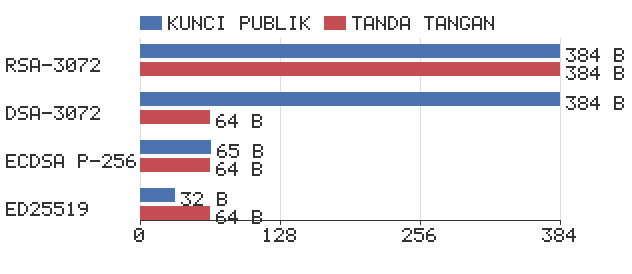
\includegraphics[width=0.98\linewidth]{figures/ukuran-tanda-tangan.png}
    \caption{Ukuran kunci publik dan tanda tangan pada tingkat keamanan yang
    setara ($\approx$ 128 bit). RSA dan DSA menuntut kunci sebesar 384 byte,
    sedangkan Ed25519 hanya 32 byte. Perhatikan pula bahwa panjang tanda
    tangan ECDSA dan Ed25519 sama --- 64 byte --- sebab keduanya menampung
    dua titik kurva, tetapi kunci publik Ed25519 setengah lebih kecil karena
    titiknya disimpan terkompresi}
    \label{fig:ukuran-tanda-tangan}
    \sumber{Ukuran bahan kriptografis mentah; gambar dibangkitkan oleh skrip
    \code{scripts/refactor/figures/ukuran\_tanda\_tangan.py} pada repositori ini.}
\end{figure}

Perbandingan itu menjelaskan arah perkembangan praktik. Ketika bandwidth dan
ruang penyimpanan belum menjadi kendala, RSA mendominasi karena verifikasinya
murah dan implementasinya sudah matang. Ketika perangkat bergerak dan
internet of things menuntut tanda tangan pada perangkat berdaya rendah,
ECDSA dan kemudian Ed25519 mengambil alih justru karena kuncinya jauh lebih
pendek, dan biaya komputasinya lebih kecil pada tingkat keamanan yang sama.

\subsection{Serangan dan Kesalahan Implementasi Lain}
Selain pemakaian ulang $k$, ada beberapa jalur serangan lain yang perlu
dikenali karena semuanya pernah berhasil pada sistem sungguhan.

\textbf{Verifikasi padding yang longgar.} Skema PKCS\#1 v1.5 menuntut agar
verifikator memeriksa seluruh struktur blok. Bila hanya sebagian yang
diperiksa, penyerang dapat menyusun blok yang lolos padahal tidak sah.
Kelas serangan ini ditemukan Daniel Bleichenbacher dan berdampak pada
beberapa implementasi besar, antara lain pustaka keamanan Mozilla dan
OpenSSL, yang kemudian diperbaiki melalui pembaruan darurat. Pelajarannya
sederhana tetapi penting: keamanan tanda tangan bergantung pada ketatnya
\emph{pemeriksaan}, bukan hanya pada kuatnya \emph{algoritma}
\citep{bleichenbacher1998}.

\textbf{Serangan galat pada penandatanganan dengan CRT.} Implementasi RSA
yang memakai Teorema Sisa Cina (CRT) untuk mempercepat penandatanganan
menghitung tanda tangan modulo $p$ dan modulo $q$ secara terpisah. Bila satu
dari kedua perhitungan itu terganggu --- misalnya oleh gangguan tegangan atau
radiasi --- dan hasilnya tetap dipakai, maka selisih antara hasil yang benar
dan hasil yang rusak mengandung faktor $p$ atau $q$. Satu tanda tangan yang
rusak sudah cukup untuk memfaktorkan modulus dan membongkar seluruh kunci
privat. Karena itu implementasi yang baik memeriksa ulang hasil CRT sebelum
mengeluarkan tanda tangan.

\textbf{Kunci yang lemah sejak pembangkitan (ROCA).} Pada tahun 2017
terungkap bahwa pustaka pembangkit kunci pada sejumlah chip Infineon ---
termasuk yang tertanam di kartu pintar, TPM, dan token perangkat keras ---
menghasilkan modulus RSA dengan struktur tersembunyi yang memungkinkan
faktorisasi jauh lebih cepat daripada seharusnya \citep{nemec2017roca}.
Kelemahan itu tidak berada pada algoritma RSA, melainkan pada cara kuncinya
dibangkitkan. Peristiwa ini menegaskan bahwa keamanan tanda tangan adalah
rantai: sekuat apa pun skema matematisnya, mata rantai terlemahnya bisa saja
berada pada pembangkit bilangan acak yang dipakai sehari-hari.
